\documentclass[a4paper,12pt,titlepage,table]{article}

\usepackage[T1]{fontenc}
\usepackage[utf8]{inputenc}
\usepackage{amsmath}
\usepackage{amsthm}
\usepackage{mathtools}
\usepackage{amsfonts}
\usepackage{amssymb}
\usepackage[margin=1in]{geometry}
\usepackage{graphicx}
\usepackage[
%hidelinks
    colorlinks
]{hyperref}
\usepackage{titlesec}
\usepackage[toc,title]{appendix}
\usepackage{algorithm}
\usepackage{algorithmicx}
\usepackage[noend]{algpseudocode}
\usepackage{cleveref}
\usepackage{newpxtext}
\usepackage[euler-digits,euler-hat-accent]{eulervm}
\usepackage{enumerate}
\usepackage[font=footnotesize,labelfont=bf]{caption}    % For figure...
\usepackage[font=footnotesize]{subcaption} % ... and subfigure
\usepackage{CJKutf8}
\usepackage[table]{xcolor}
\usepackage{pgfplots}
\usepackage{pdflscape}
\usepackage{multirow}
\usepackage{hhline}
\usepackage{tabularray}
\usepackage{bera}% optional: just to have a nice mono-spaced font
\usepackage{listings}

% We will externalize the figuresa
\usepgfplotslibrary{external}
\pgfplotsset{compat = 1.15}
\tikzexternalize[prefix=build/]
\usepackage{fp}
\usetikzlibrary{fixedpointarithmetic}

\author{Mateusz Maćkowski}
\title{Implementation of Context Binning and Model Clustering for Compression
of Genetic Data}
\date{August 2022}

\hypersetup{pdfinfo={
    Title={Implementation of Context Binning and Model Clustering for
    Compression of Genetic Data},
    Author={Mateusz Maćkowski}
}}

\newcommand{\sectionbreak}{\clearpage}

% Useful definitions
\newcommand{\biggO}[1]{\mathcal{O}\left(#1\right)}
\newcommand{\bigO}[1]{\mathcal{O}(#1)}
\newcommand{\bigOTilde}[1]{\tilde{\mathcal{O}}(#1)}
\newcommand{\substr}{\preceq}
\newcommand{\superstr}{\succeq}
\newcommand\boxedletter[1]{\text{%
    \tikz[baseline=(X.base)]
    \node (X) [draw, inner sep=0, minimum size=1.2em, rounded corners] {$#1$};}}
\newcommand{\word}{\overline}
\newcommand{\setR}{\mathbb{R}}
\newcommand{\setN}{\mathbb{N}}
\newcommand{\setQ}{\mathbb{Q}}
\newcommand{\setZ}{\mathbb{Z}}
\newcommand{\setC}{\mathbb{C}}

\theoremstyle{plain}

\begin{document}
    \hypersetup{pageanchor=false}
    \thispdfpagelabel{a}
    \begin{titlepage}
  \setlength{\parindent}{0pt}
  \setlength{\parskip}{0pt}
  \makeatletter
  \def\myhrulefill{\leavevmode\leaders\hrule height 1pt\hfill\kern\z@}
  \makeatother

  \centering

  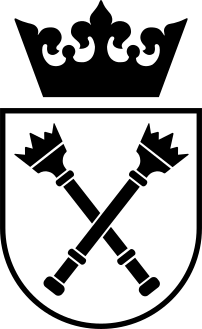
\includegraphics[scale=0.3]{img/herb_uj.pdf}

  \vspace{0.5em}

  \Large
  \textbf{Jagiellonian University}\\
  \large
  Faculty of Mathematics and Computer Science\\
  Institute of Computer Science
  \normalsize

  \vspace{4em}

  \large
  \makeatletter
  \textbf{\@author}
  \makeatother
  \\
  \normalsize
  Student ID: 1136132

  \vspace{4em}

  \myhrulefill\\
  \huge
  \makeatletter
  \textbf{\textsc{
    \@title
  }}
  \makeatother
  \\
  \vspace{-0.5em}
  \myhrulefill

  \normalsize
  \vspace{4em}

  \large
  Master's Thesis\\
  Computer Science

  \vfill

  \large
  Supervisor:\\
  \textbf{Dr. Jarosław Duda}\\
  \normalsize
  \vspace{4em}
  \makeatletter
  Kraków, \@date
  \makeatother
\end{titlepage}

    \pagenumbering{Alph}
    \thispdfpagelabel{b}
    \begin{abstract}
    In recent years, there happened a gigantic leap in the speed of DNA sequencing methods, which allowed us to sequence DNAs of complex organisms, such as humans, quickly.
    However, this leads to increasing demand for disk storage, as the sizes of the databases containing such data can easily reach dozens of terabytes.
    In his article ``Context binning, model clustering and adaptivity for data compression of genetic data'', Jarek Duda proposes promising compression techniques that should help build a compressor better than the current state of the art.
    This thesis describes the compressor built to evaluate those techniques, tests it with real-world data and compares it to other genetic data compression tools.
\end{abstract}


    \hypersetup{pageanchor=true}
    \pagenumbering{roman}
    \tableofcontents
    \newpage
    \pagenumbering{arabic}

    \section{Introduction}\label{sec:introduction}

The rapid growth of bioinformatics databases leads to the increasing demand
for disk storage.
In recent years, there happened a gigantic leap in the speed of DNA
sequencing methods, which allowed us to sequence DNAs of complex organisms,
such as humans, quickly\cite{Ashley2016}.
However, this leads to increasing demand for disk storage, as the sizes of
the databases containing such data can easily reach dozens of terabytes.

Therefore, it seems that it could be very beneficial to try to compress the
sequences, hoping to make some savings and avoid needing to store such vast
amounts of data.
It seems that the choice of FASTQ compression tools is quite
limited at the moment, so one can expect some improvements in both
compression ratio and speed are possible.

In his article ``Context binning, model clustering and adaptivity for data
compression of genetic data''\cite{https://doi.org/10.48550/arxiv.2201.05028},
Jarek Duda proposes promising compression techniques that should help build a
compressor better than the current state of the art.
In order to allow real-world evaluation of those
techniques, a compressor called \emph{idencomp} has been built.
This article focuses on this compressor's implementation details and its
evaluation with some real-world data.

    \section{Problem description}\label{sec:problem-description}

We would like to be able to compress a DNA sequence read from a
FASTQ\cite{fastq} file containing both the acids and quality scores so that
it takes less space while getting a better compression rate/speed ratio than
other widely used compression methods.
In other words, we have a set of sequences \((a_i, q_i)_{i=1}^N\), where \(a_i\)
is an acid (i.e., $a_i \in \{\mathtt{A}, \mathtt{C}, \mathtt{T}, \mathtt{G},
\mathtt{N}\}$, where \texttt{N} is an invalid nucleotide), and \(q_i\) is a
quality score (a non-negative integer up to between 40 and 94, depending on
the sequencing method), and want to compress it.

A popular approach is encoding the data \emph{symbol-by-symbol}, using a
conditional
distribution of the following symbol based on a few previous ones or possibly
some other context information.
With an accurate entropy coder, such as Asymmetric Numeral Systems (ANS)\cite{7170048}, a
symbol of probability \(p\) requires \(\log_2(1/p)\) bits to be encoded.
Hence, by combining such a statistical model with ANS, a compressor would
achieve a close-to-entropy compression ratio.

The compressor could be equipped with a set of commonly used statistical
models so that they would not need to be a part of the compressed file.
It also should allow using some external models if needed for flexibility.
The decompressor should be able to use those standard models and display an
error message if an unknown model appears in a specific file.
Also, the compressor should be able to automatically choose the model best
matching the currently processed sequence so that it takes as little disk
space as possible.
Also, both the compressor and decompressor could use multiple CPU threads to
make the file processing faster.

    \section{Implementation}\label{sec:implementation}

\subsection{Overview}\label{subsec:overview}

\emph{idencomp} (jap.\hspace{0.2em}\begin{CJK}{UTF8}{min}
                                       遺伝コンプレッサー
\end{CJK}
(\emph{idenkonpuressa}) --- ``genetic compressor'') is an open-source genetic
data
compressor built for the needs of this article.
It was written in the Rust programming language\cite{rust} because it combines
versatility, high performance, ease of use, and support for generics.
The compressor has been built for modern multi-core CPUs; hence it can use
multiple CPU threads for all the critical parts.

For compressing the sequence data (acids and quality scores), the compressor
uses \emph{rANS} (the range variant of asymmetrical numerical systems)\cite{7170048}
combined with \emph{context binning} and \emph{\(k\)-means model clustering}
described in \Cref{subsec:context-binning} and
\Cref{subsec:$k$-means-model-clustering}, respectively.
For storing the sequence names, \emph{idencomp} can use
\emph{Deflate}\cite{rfc1951} or
\emph{Brotli}\cite{rfc7932}, depending on the compression quality option.
The compressor stores the compressed sequences in a custom binary data
format, while the models are serialized using \emph{MessagePack}\cite{messagepack}.

The compressor has been built with high code quality, is thoroughly
documented, includes an extensive test suite, and uses a CI infrastructure to
execute builds, tests, and benchmarks.
The project has been divided into a CLI interface and an accompanying library.
The entire compressor source code has been published on the GitHub
platform\cite{idencomp} under the terms of the MIT license, so it is free to be
used and modified by other researchers.
Because of the lack of rANS implementations/bindings library for Rust, one
called \emph{rans} has also been developed and published\cite{rans-rs} that uses
\emph{ryg\_rans}\cite{ryg-rans} implementation written in C programming language under the hood.

\subsection{Context binning}\label{subsec:context-binning}

A statistical model based on previous symbols, while very appealing for our
use case and promising a good compression ratio, has a considerable
disadvantage: it can quickly get huge.
Using big models not only hurts the disk storage but also affects the
performance --- when an entire model cannot fit the CPU cache, the performance
may worsen significantly.
Hence, we would like to make models smaller by combining the contexts into
some disjoint subsets.

The idea for fixing this problem, proposed by Jarek Duda
in~\cite{https://doi.org/10.48550/arxiv.2201.05028}, is called context binning.
For any two contexts, the cost of merging them is the difference between the
merged context rate multiplied by its probability and the sum of source
context rates multiplied by their probabilities.
Using this equality, one can use a greedy search algorithm to optimally bin
the contexts while maintaining the best possible compression rate.

The algorithm below presented in~\cite{https://doi.org/10.48550/arxiv.2201.05028} computes, for a given set of
contexts $C$ and cost function $\Delta: C \times C \rightarrow \mathbb{R}$,
a binary tree representing an optimal binning.

\algnewcommand{\True}{\textbf{true}}
\algnewcommand{\False}{\textbf{false}}
\algnewcommand{\Null}{\textbf{null}}
\algnewcommand{\Let}{\textbf{let }}
\algnewcommand{\To}{\text{ to }}

\begin{algorithm}[H]
    \caption{Greedy algorithm for finding optimal binning of contexts}%
    \label{alg:binning}%
    \begin{algorithmic}%
        \State\Comment{Binary tree node is a tuple (context, available,
            left-child, right-child)}%

        \Procedure{Context-Binning}{$C$}%
            \State\Comment{$C = (c_i)_{i=1}^N$ is a list of contexts}%
            \State{\Let $T = (c_i, \True, \Null, \Null)_{i=1}^N$ be the
            initial list of nodes (leaves)}
            \State{\Let $Q$ be an empty priority queue of pairs of indices in
                $T$}
            \For{$i \gets 1 \To N$}
                \For{$j \gets i + 1 \To N$}
                    \State{$\Call{Push}{Q, (i, j), \Delta(T[i].\text{context}, T[j].\text{context})}$}
                \EndFor
            \EndFor
            \For{$k \gets N + 1 \To 2N-1$}
                \State{$(i, j)\gets\Call{Pop-Active}{Q, T}$}
                \State{$T[i].\text{available} \gets \False$}
                \State{$T[j].\text{available} \gets \False$}
                \State{\Let $c$ be a new context made by merging $T[i]
                .\text{context}$ and $T[j].\text{context}$}
                \State{$v \gets (c, \True, i, j)$}
                \State{$\Call{Append}{T, v}$\Comment{at index $k$}}
                \For{$l \gets 1 \To k - 1$}
                    \State{$\Call{Push}{Q, (l, k), \Delta(T[l].\text{context}, T[k].\text{context})}$}
                \EndFor
            \EndFor
            \State{\Return{$T$}}
        \EndProcedure%

        \Procedure{Pop-Active}{$Q$, $T$}%
            \State\Comment{$Q$ is a priority queue of pairs of indices in array $T$}%
            \State\Comment{$T$ is an array of nodes, as described above}

            \Repeat
                \State{$(i, j)\gets\Call{Pop}{Q}$}
            \Until{$T[i].\text{available} \textbf{ and } T[j].\text{available}$}
            \State\Return{$(i, j)$}
        \EndProcedure
    \end{algorithmic}%
\end{algorithm}

The main problem with using the greedy algorithm is that its computational
and memory complexity is $\bigOTilde{n^2}$.
Because of that, \emph{pre-binning} has been implemented as well: before doing
the proper binning, we bin the configurable number of the least probable
contexts into one, ignoring the cost of merging them completely.
While this harms the compression rate of resulting models, it should make the
computation time slightly more bearable, especially for more sizeable models.

\subsection{$k$-means model clustering}\label{subsec:$k$-means-model-clustering}

A single statistic model for the entire file may not be optimal for
compressing the entire file.
Hence, we might want to use multiple of them and select the one providing the
smallest compressed data size for each sequence individually.
In order to do that, we need to choose a few models to be used across the
entire file first.

An idea proposed by Jarek Duda in~\cite{https://doi.org/10.48550/arxiv.2201.05028} is an adaption of the
$k$-means algorithm: here,
the ``observations'' are sequences, and the ``cluster centroids'' are models.
We use this algorithm to choose a subset of models best suited for the file,
which we then put in the file header.
To make this choice fast, we do it based on the first few megabytes of the
file, assuming they share similar statistics as the rest of it.
After this initialization step, we test each sequence with those selected
models and use the best model for each.

\begin{algorithm}[H]
    \caption{$k$-means clustering adapted for choosing a subset of models to
    use for the file}%
    \label{alg:kmeans}%
    \begin{algorithmic}%
        \Procedure{K-Means}{$k$, $M$, $S$}%
            \State\Comment{$k$ is an requested number of clusters}%
            \State\Comment{$M$ is a collection of models}%
            \State\Comment{$S$ is a collection of sequences}%
            \State{\Let $(s_i)_{i=1}^k$ be a random subset of $S$ of size $k$}
            \State{$R\coloneqq(R_i)_{i=1}^k \gets (\{s_i\})
            _{i=1}^k$\Comment{$R$ is a disjoint covering of some subset of $S$}}
            \State{$m\coloneqq(m_i)_{i=1}^k \gets \Call{Find-Means}{M, R}$}
            \Repeat
                \For{$i \gets 1 \To |S|$}
                    \State{\Let $m_j$ be the best model for $S_i$ from $m$}
                    \State{cover $S_i$ with $R_j$}
                \EndFor
                \State{$(m_i)_{i=1}^k \gets \Call{Find-Means}{M, R}$}
            \Until{$R$ has not changed}
            \State{\Return{$m$}\Comment{at this point, $R$ covers the entire
                $S$}}
        \EndProcedure%
    \end{algorithmic}%
\end{algorithm}

\subsection{Compression/decompression using rANS}\label{subsec:compression
/decompression-using-rans}
The sequences are compressed with rANS, using prior acids and quality scores
to compute the current context.
Also, the compressor interleaves the outputs of two separate rANS encoders
(one for acids and one for quality scores) into the same data buffer.
Interleaving prevents CPU pipeline stalls by removing some immediate data
dependencies.

\subsection{Contexts}\label{subsec:contexts}
The base of the compression algorithm used in the compressor is the context -
the list of local symbol probabilities at a given position in the file.
In this article, a \emph{context} will mean such list of symbol probabilities,
and a \emph{context specifier} will be the description of a context itself - for
example, [\texttt{A}: 20\%; \texttt{C}: 30\%; \texttt{G}: 40\%; \texttt{T}:
10\%] is a context, and [3
previous acids: \texttt{A}, \texttt{C}, \texttt{G}; 2 previous quality
scores: 39, 40] is a context
specifier.

\emph{idencomp} uses Rust’s powerful generics system to rapidly define
various types
of context specifiers while still maintaining high performance.
There are three distinct context specifiers: \emph{dummy}, \emph{generic},
and \emph{light}.

The \emph{dummy context specifier} treats the entire sequence as having the same
context.
The dummy context is mainly used for tests and comparing various context
specifiers to some base.

The \emph{generic context specifier} contains $N$ previous acids (including
\texttt{N} - ``invalid
read''), $M$ previous quality scores, and $P$ bits to store the position in the
file.
Because this context specifier stores the quality scores as defined in the
FASTQ file, it can lead to generating huge models, as the format supports up
to 94 different quality scores.
The generic context specifier may generate up to $5^N \cdot 94^M \cdot 2^P$
distinct
contexts.
The dummy context specifier described above can be defined as a generic
context specifier with $N$, $M$, and $P$ equal to 0.

The \emph{light context specifier} contains $N$ previous acids, $M$ previous
quality scores (between 0 and $Q_{\text{max}}$ each), and $P$ bits to store the
position in the file.
The difference between generic context specifier is that the light
variant quantizes the quality scores and replace \texttt{N} (invalid) acids with
an \texttt{A} acid and the quality score of 0.
This context specifier can produce much smaller models while maintaining a
decent compression ratio.
Specifically, this context specifier may generate up to
$4^N \cdot {Q_\text{max}}^M \cdot 2^P$ contexts.

\subsection{Model data format}\label{subsec:model-data-format}

Because the model data does not need to be very concise, \emph{MessagePack}
has been
chosen as the data storage format for the models.
A model file contains the model type (acids or quality scores), context
specifier type (described in \Cref{subsec:contexts}), list of contexts
(symbol probabilities), and map of context specifiers to context indices.
\emph{idencomp} preprocesses that data (for example, by removing any uses of
floating-point values) before using it with the rANS coder to achieve the
best performance.

Please see \Cref{sec:model-data-format} for more detailed information about the
model data format.

\subsection{Sequence data format}\label{subsec:sequence-data-format}

\emph{idencomp} uses a custom binary format (\emph{IDN}) to store the
compressed sequence
data to achieve parallelism, high data density, and high customizability.
The IDN format was inspired by the CRAM data format\cite{cram} but is much
simpler and
lightweight, but at the same time, it only allows for storing a more limited
set of data.

Any IDN file consists of a file header, metadata, and an arbitrary number of
blocks.
Currently, only one type of metadata item is supported: model identifiers,
which indicate which models a file uses, to allow the decompressor to load
the corresponding models (or throw an error if they are unavailable).

A data block is a container for slices.
Each slice is either a ``switch model'' slice that instructs the decompressor
to use a specific model for the subsequent sequences or a ``sequence'' slice,
which is a compressed sequence data.
The sequence slice contains both acids and quality scores in a single data
stream.

The sequence names may also appear in a file unless the user has chosen not
to include them.
However, since compressing sequence identifiers is well-researched in other
compressors, this article focuses entirely on compressing the sequence data.
Hence, the input data used in the tests will not contain any sequence names.

The blocks are defined mainly to allow compression and decompression
parallelism.
Each block can be compressed and decompressed independently, so it is
possible to process each block in a separate CPU thread and then combine the
results.
Blocks enable the compressor and decompressor to use virtually any number of
threads.

Please see \Cref{sec:idn-data-format} for more detailed information about the
IDN format.

\subsection{Command-Line Interface}\label{subsec:command-line-interface}

The Command-Line Interface (CLI) is the primary way of interacting with the
compressor.
It has four main modes of operation, which are being made use of in this
article:

\begin{itemize}
    \item \emph{Model generation} --- reads a given FASTQ file and generates model(s)
    using statistics calculated from that file.
    This mode can optionally generate models for all defined context specifiers
    in separate CPU threads.
    It also has a context number limiter to avoid generating models too big to
    be used in practice.
    \item \emph{Context binning} --- reads a given model and generates a binned
    version of it.
    Can optionally generate N versions of equally distributed context numbers in
    separate CPU threads.
    \item \emph{Compression} --- compresses a given FASTQ file into an IDN file.
    Can optionally use multithreading to compress multiple blocks in parallel.
    \item \emph{Decompression} --- decompresses a given IDN file into a FASTQ file.
    Can optionally use multithreading to decompress multiple blocks in parallel.
\end{itemize}

The compressor’s documentation describes more CLI options that are available.
The article will present the same command line options used to do the
described tests.

    \section{Evaluation and comparison with other FASTQ compression tools}\label
{sec:evaluation-and-comparison-with-other-fastq-compression-tools}

\subsection{Models}\label{subsec:models}

All the predefined models used in the tests below have been created using
publicly-available sequences processed by \emph{idencomp}.
The process for generating each model has followed the procedure below:

\begin{enumerate}
    \item Download the sequence and convert it to a FASTQ file.
    \item Use the \texttt{generate-models-all} \emph{idencomp} command to
    create the models for all possible context specifier types.
    \item By analyzing the statistics generated by \emph{idencomp}, choose
    the model which achieves the best compression rate and is not too big to
    be further processed.
    Choose one model for acids and one for quality scores.
    \item Use the \texttt{bin-contexts-all} \emph{idencomp} command to
    generate binned versions of the chosen models.
    \item By analyzing the statistics, choose the model significantly smaller
    than the original but still achieving a decent compression rate.
\end{enumerate}

\begin{figure}[h]
    \centering
    \begin{tikzpicture}
    \pgfplotsset{
        table/search path={data},
    }

    \begin{semilogyaxis}
    [
        xlabel={Number of contexts},
        ylabel={Rate penalty [bpv]},
        xmin=0, xmax=27520,
        ymin=0, ymax=0.5,
        xmajorgrids = true,
        xminorgrids = true,
        minor x tick num=4,
        ymajorgrids = true,
        yminorgrids = true,
        height = 8cm,
        width = 12cm,
        max space between ticks=40,
        log number format code/.code={%
            \begingroup
            \pgfset{fixed point arithmetic,
                number format/.cd, fixed relative, precision=2}%
            \pgfmathparse{exp(#1)}%
            \pgfmathprintnumber{\pgfmathresult}%
            \endgroup
        },
        scaled x ticks=false,
        grid style=dashed
    ]

        \addplot+ [color=blue, only marks, mark=*, mark size=1pt] table [x=context number, y=rate, col sep=comma] {binning.csv};
    \end{semilogyaxis}
\end{tikzpicture}


    \caption{Relationship between number of contexts and compression rate
    penalty for all binned versions of the quality scores model generated
    from the sample SRR16141966}
    \label{fig:binning-example}
\end{figure}

\Cref{fig:binning-example} shows the relationship between the number of
contexts and the compression rate.
The compression rate here is expressed as the penalty relative to the
original, unbinned model.
Notice that the bits-per-value differences between the binned versions are
most significant at the low number of bins (up to a few hundred contexts) and
get very small later;
this is true for virtually all tested models.
Usually, there are a few compression rate penalty spikes between binned
versions in the middle (as can be seen around context number 21,000 here).
The binned versions just after those spikes might be good candidates to be
used as the final, compact versions of the model.
In this specific case, the model with 463 contexts was kept --- as one can
see on the plot, there is a spike there as well.

All of the pre-defined model details can be seen in
\Cref{sec:pre-defined-models}.
Notice that some models achieve excellent compression rates even though they
are tens of times smaller than the originals, and some require to be kept
large to avoid harming the rate too much.

\subsection{Test details}\label{subsec:test-details}

The tests consider the compression ratio and compression/decompression speed
(and the relationship between those values).
We define the compression speed as the original data size divided by the
processing time.
The same applies to the decompression speed (resulting file size divided by
the decompression time).
The tests do not take model sizes into account --- however, they are
insignificant in most cases, as most of the tests are performed on 1GB files,
while all of the models take about 30MB of disk space.
Please consult \Cref{sec:benchmarking-tools-and-environment} for the exact
testing environment and the tools that are tested.

\newpage

\subsection{Small sample}\label{subsec:small-data}

The test with a small file (first 10MB of SRR19549058) shows that the
preprocessing of models takes a significant time and overwhelms any other
processing cost.
The compressor and decompressor load all models before processing the file,
which means there is an almost constant startup delay.
Therefore, while compression speed is on par with \emph{gzip}, decompression
is much slower.

\begin{figure}[h]
    \begin{subfigure}{\textwidth}
        \centering
        \input{img/bench-small-data-compress}
        \caption{Compression}
    \end{subfigure}
    \begin{subfigure}{\textwidth}
        \centering
        \vspace{1em}
        \begin{tikzpicture}
    \tikzstyle{every node}=[font=\small]
    \pgfplotsset{
        table/search path={data},
    }

    \begin{semilogxaxis}
    [
        xlabel={Speed [MB/s]},
        ylabel={Ratio},
        xmin=0.5, xmax=400,
        ymin=3.8, ymax=6.5,
        xmajorgrids = true,
        xtick = {1, 2, 4, 8, 16, 32, 64, 128, 256},
        ymajorgrids = true,
        scaled x ticks=false,
        log number format code/.code={%
        \begingroup
        \pgfset{fixed point arithmetic,
            number format/.cd, fixed relative, precision=3}%
        \pgfmathparse{exp(#1)}%
        \pgfmathprintnumber{\pgfmathresult}%
        \endgroup
        },
        height = 8cm,
        grid style=dashed
    ]

        \addplot+ [
            only marks,
            mark=*,
            nodes near coords*={\Label},
            visualization depends on={value \thisrow{cmd} \as \Label},
            visualization depends on={value \thisrow{decompress_anchor} \as \myanchor},
            every node near coord/.append style={anchor=\myanchor}
        ] table [
            x expr={\thisrow{decompress_speed} / 1000000},
            y expr={1 / \thisrow{ratio}},
            col sep=comma
        ] {small-data.csv};
    \end{semilogxaxis}
\end{tikzpicture}


        \caption{Decompression}
    \end{subfigure}
    \caption{%
        Compressor benchmark for the first 10MB of SRR19549058
    }
    \label{fig:bench-small-data}
\end{figure}

\newpage

\subsection{Sample with a dedicated model}\label{subsec:sample-with-a
-dedicated-model}

This test has been performed using the first 1GB of sample SRR2962693, which
has a dedicated model in \emph{idencomp}.
Because the input data is much larger than in the previous test, the startup
time is not significant anymore.

\emph{idencomp} performs similarly to the other general compressors (like
\emph{gzip} and \emph{bzip2}), but worse than dedicated sequence compressing
tools, both in terms of performance and compression ratio.
It also seems that \texttt{{-}{-}quality=1} option (which reduces the number
of models used during compression) works pretty well here.
There is rarely more than one model needed to compress a sequence, so the
mentioned option improves the performance almost without harming the
compression ratio.

\begin{figure}[h]
    \begin{subfigure}{\textwidth}
        \centering
        \input{img/bench-dedicated-model-compress}
        \caption{Compression}
    \end{subfigure}
    \begin{subfigure}{\textwidth}
        \centering
        \vspace{1em}
        \input{img/bench-dedicated-model-decompress}
        \caption{Decompression}
    \end{subfigure}
    \caption{%
        Compressor benchmark for the first 1GB of SRR2962693
    }
    \label{fig:bench-dedicated-model}
\end{figure}

\newpage

\subsection{Unknown sample with a known sequencing method}
\label{subsec:sample-with-a -known-sequencing-method}

This test has been performed using the first 1GB of sample SRR2747516.
This sample does not have a dedicated model, but is similar to other known
samples --- it's a sequencing of a mammal (Shiba Inu dog) that has been
performed using Illumina HiSeq 2500.

\emph{idencomp} performs slightly worse here in the terms of the compression
ratio.
It's worse than general compression tools as well.
The performance is comparable both with general-purpose and dedicated
compression tools, however.

\begin{figure}[h]
    \begin{subfigure}{\textwidth}
        \centering
        \input{img/bench-known-sequencing-compress}
        \caption{Compression}
    \end{subfigure}
    \begin{subfigure}{\textwidth}
        \centering
        \vspace{1em}
        \input{img/bench-known-sequencing-decompress}
        \caption{Decompression}
    \end{subfigure}
    \caption{%
        Compressor benchmark for the first 1GB of SRR2747516
    }
    \label{fig:bench-known-sequencing}
\end{figure}

\newpage

\subsection{Best performance}\label{subsec:best-performance}

This test aims to improve the performance.
It has been performed using the first 1GB of sample SRR5373739.
This sample has a dedicated tiny model (eight acid contexts and six quality
score contexts), so that it can easily fit into the CPU cache.
\emph{idencomp} has been forced to use this specific model by removing all
other models, so the startup time is also lower.
In addition to that, the block size has been increased, which seems to
improve performance with large files.

While \emph{idencomp} does not achieve the best compression ratio, the
performance is excellent.
It outperforms almost all other tools in compression speed, and maintains a
decent decompression speed as well.

\begin{figure}[h]
    \begin{subfigure}{\textwidth}
        \centering
        \input{img/bench-best-performance-compress.tex}
        \caption{Compression}
    \end{subfigure}
    \begin{subfigure}{\textwidth}
        \centering
        \vspace{1em}
        \begin{tikzpicture}
    \tikzstyle{every node}=[font=\small]
    \pgfplotsset{
        table/search path={data},
    }

    \begin{semilogxaxis}
    [
        xlabel={Speed [MB/s]},
        ylabel={Ratio},
        xmin=2, xmax=1500,
        ymin=4, ymax=10,
        xmajorgrids = true,
        xtick = {1, 2, 4, 8, 16, 32, 64.005, 128, 256, 512, 1024, 2048},
        ymajorgrids = true,
        scaled x ticks=false,
        log number format code/.code={%
        \begingroup
        \pgfset{fixed point arithmetic,
            number format/.cd, fixed relative, precision=4}%
        \pgfmathparse{exp(#1)}%
        \pgfmathprintnumber{\pgfmathresult}%
        \endgroup
        },
        height = 8cm,
        grid style=dashed
    ]

        \addplot+ [
            only marks,
            mark=*,
            nodes near coords*={\Label},
            visualization depends on={value \thisrow{cmd} \as \Label},
            visualization depends on={value \thisrow{decompress_anchor} \as \myanchor},
            every node near coord/.append style={anchor=\myanchor}
        ] table [
            x expr={\thisrow{decompress_speed} / 1000000},
            y expr={1 / \thisrow{ratio}},
            col sep=comma
        ] {best-performance.csv};
    \end{semilogxaxis}
\end{tikzpicture}


        \caption{Decompression}
    \end{subfigure}
    \caption{%
        Compressor benchmark for the first 1GB of SRR5373739.
    }
    \label{fig:bench-best-performance}
\end{figure}

\newpage

\subsection{Better compression ratio}\label{subsec:better-ratio}

The last test tries to improve the compression ratio without hurting the
performance built in the previous test.
As before, \emph{idencomp} uses a tiny model built specifically for a file
--- this time, sample SRR2962693 is reused, but the model has been built
using only the first gigabyte of the file.
The second gigabyte is used as a test file to be compressed.

The main reason for the poor compression ratio of \emph{idencomp} is that
every single sequence takes about nine additional bytes for the headers to be
serialized, most of which is occupied by the length of a sequence, both
compressed and uncompressed.
In practice, all the sequence lengths in a single file are usually equal (as
in SRR2962693, where each sequence has a length of 126).
Therefore, this test uses an evaluation file modified to our advantage ---
the subsequent sequences are glued together until they are at least 10000
symbols long.
This modified file is then compressed.

\emph{idencomp} performs really well here.
Not only is it faster than almost all other compression tools, it also
maintains a compression ratio better than all general-purpose compressors.
Other dedicated compression methods achieve similar compression ratio.
See \Cref{fig:bench-better-ratio} for the details.

\begin{figure}[h]
    \begin{subfigure}{\textwidth}
        \centering
        \input{img/bench-better-ratio-compress.tex}
        \caption{Compression}
    \end{subfigure}
    \begin{subfigure}{\textwidth}
        \centering
        \vspace{1em}
        \begin{tikzpicture}
    \tikzstyle{every node}=[font=\small]
    \pgfplotsset{
        table/search path={data},
    }

    \begin{semilogxaxis}
    [
        xlabel={Speed [MB/s]},
        ylabel={Ratio},
        xmin=4, xmax=1024,
        ymin=3, ymax=7,
        xmajorgrids = true,
        xtick = {1, 2, 4, 8, 16, 32, 64.005, 128, 256, 512, 1024, 2048},
        ymajorgrids = true,
        scaled x ticks=false,
        log number format code/.code={%
        \begingroup
        \pgfset{fixed point arithmetic,
            number format/.cd, fixed relative, precision=4}%
        \pgfmathparse{exp(#1)}%
        \pgfmathprintnumber{\pgfmathresult}%
        \endgroup
        },
        height = 9cm,
        grid style=dashed
    ]

        \addplot+ [
            only marks,
            mark=*,
            nodes near coords*={\Label},
            visualization depends on={value \thisrow{cmd} \as \Label},
            visualization depends on={value \thisrow{decompress_anchor} \as \myanchor},
            every node near coord/.append style={anchor=\myanchor}
        ] table [
            x expr={\thisrow{decompress_speed} / 1000000},
            y expr={1 / \thisrow{ratio}},
            col sep=comma
        ] {better-ratio.csv};
    \end{semilogxaxis}
\end{tikzpicture}


        \caption{Decompression}
    \end{subfigure}
    \caption{%
        Compressor benchmark for the second gigabyte of SRR2962693.
    }
    \label{fig:bench-better-ratio}
\end{figure}

    \section{Conclusion and further work}\label{sec:conclusion-and-further-work}

This thesis has presented a few ways to improve compressing the DNA sequence
data.
It described an implementation of context binning, $k$-means model clustering,
and how they can be combined with already known solutions such as entropy
coders (rANS) by creating a working compressor prototype and a custom data
format.
The compressor has been tested on real-world data and compared with other
widely-used tools.

The compressor performs pretty well, especially when compared to generic data
compressor tools.
It is usually much faster than most of the competitors, and can maintain a
decent compression ratio, too.
The proposed methods are quite promising and worth further research,
especially by incorporating them into existing, well-developed tools.
This thesis, however, focused on building a new solution from scratch, so it
can be seen how well it can perform while eliminating as many other external
factors as possible.

That being said, many improvements are emerging right now:

\begin{itemize}
    \item The model format is not very concise - in fact, it is built upon a
    generic format to reduce the implementation time.
    Instead, we could use a custom binary data format and do the
    preprocessing step currently done at \emph{idencomp} startup before
    saving the model, so it does not need to be done again later.
    This would improve the performance and possibly make the models smaller
    as well.
    \item The IDN file format is quite verbose as well.
    Although it is a custom format explicitly built for this purpose, it is
    not very compact.
    The main problem is that every single sequence is stored as a separate
    slice in a block.
    This separation adds overhead for each sequence because its length and
    the slice size need to be stored uncompressed and because the compressor
    resets the rANS coder state, losing the fractional bits that it could use
    otherwise.
    Instead, we could first concatenate all the sequences for each block and
    store their lengths separately --- similarly to what has been done in
    \Cref{subsec:better-ratio}.
    We could compress the lengths as well --- even simple
    RLE\cite{Salomon2007-bj} compression would probably suffice here, as
    the read length is equal through the entire file in most real-world data.
    \item The compressor tests all the chosen models for each sequence.
    Those tests are not done very efficiently, as the compressor uses the
    actual rANS encoder.
    It could instead calculate the expected number of bytes using the
    \(\log_2(1/p)\) formula, which should be much quicker.
    \item The greedy context binning algorithm is relatively slow, especially
    for bigger models.
    Because of its computational and memory complexity, it is almost unusable
    for models with more than tens of thousands of contexts.
    It would be nice to develop a heuristic/probabilistic algorithm to use
    bigger models efficiently and see possible improvements.
    \item The model could be generated for a specific file instead of relying
    on predefined models.
    This would dramatically improve the compression ratio for unknown samples.
    However, this would require a faster context binning algorithm and some
    automatic method for choosing the best fitting context specifier.
    \item Many other low-level performance improvements are possible as well.
    For example, the underlying rANS implementation is not very fast and
    could be replaced with a faster one (or even rewritten from scratch just
    for this purpose).
\end{itemize}


    \bibliographystyle{acm}
    \bibliography{bibliography}

    \begin{appendices}
        \crefalias{section}{appendix}
        \section{IDN data format}\label{sec:idn-data-format}

The IDN file starts with \texttt{IDENCOMP} bytes encoded in ASCII, followed
by the version number (currently always 1).
Then, there is the metadata section, which contains the number of metadata
items and the items themselves.
Currently, only one type of metadata item is supported: model identifiers,
which indicate which models a file uses, to allow the decompressor to load
the corresponding models (or throw an error if they are unavailable).

The file header is followed by an arbitrary number of data blocks.
The data block header consists of the compressed data length and
CRC32\cite{rfc3385} checksum of all the sequence data in a block.
Then, it is followed by an arbitrary number of slices.

Each slice is either a ``switch model'' slice that instructs the decompressor
to use a specific model for the subsequent sequences or a ``sequence'' slice,
which is a compressed sequence data.
For completeness, the sequence identifiers (names) may also appear in a file
as a separate slice, containing all of the sequence names separated by
newlines, and compressed using either Deflate (for lower compression quality
options) or Brotli (for higher).

\begin{figure}[!ht]
    \centering
    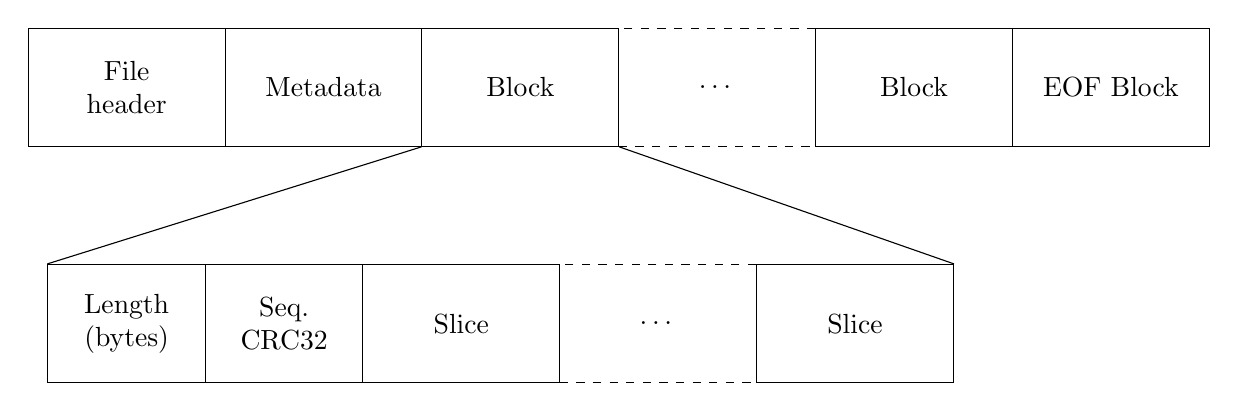
\begin{tikzpicture}[transform shape]
    \node at (0,3) [minimum height=1.5cm,minimum width=2.5cm,draw,align=center] (header) {File\\header};
    \node at (2.5,3) [minimum height=1.5cm,minimum width=2.5cm,draw] (metadata) {Metadata};
    \node at (5,3) [minimum size=1.5cm,minimum width=2.5cm,draw] (b1) {Block};
    \node at (7.5,3) [minimum height=1.5cm,minimum width=2.5cm,style=dashed,draw,inner sep=0] (b2) {\ldots};
    \node at (10,3) [minimum height=1.5cm,minimum width=2.5cm,draw] (b3) {Block};
    \node at (12.5,3) [minimum size=1.5cm,minimum width=2.5cm,draw] (beof) {EOF Block};

    \node at (0,0) [minimum height=1.5cm,minimum width=2cm,draw,align=center] (b_length) {Length\\(bytes)};
    \node at (2,0) [minimum height=1.5cm,minimum width=2cm,draw,align=center] (b_checksum) {Seq.\\CRC32};
    \node at (4.25,0) [minimum height=1.5cm,minimum width=2.5cm,draw] (slice1) {Slice};
    \node at (6.75,0) [minimum height=1.5cm,minimum width=2.5cm,style=dashed,draw,inner sep=0] (slice2) {\ldots};
    \node at (9.25,0) [minimum size=1.5cm,minimum width=2.5cm,draw] (slice3) {Slice};

    \draw (b1.south west) -- (b_length.north west);
    \draw (b1.south east) -- (slice3.north east);
\end{tikzpicture}

    \caption{%
        High-level diagram of the IDN file format
    }
    \label{fig:idn-file-format}
\end{figure}

        \section{Model data format}\label{sec:model-data-format}

Because the model data does not need to be very concise, MessagePack has been
chosen as the data storage format for the models.
The file contains the model type (acids or quality scores), context specifier
type (described in \Cref{subsec:contexts}), list of contexts (symbol
probabilities), and map of context specifiers to context indices.
Precisely, the data stored in such MessagePack file corresponds to a given
JSON file:

\colorlet{punct}{red!60!black}
\definecolor{background}{HTML}{EEEEEE}
\definecolor{delim}{RGB}{20,105,176}
\colorlet{numb}{magenta!60!black}

\lstdefinelanguage{json}{
    basicstyle=\normalfont\ttfamily,
    numberstyle=\scriptsize,
    commentstyle=\color{gray},
    stepnumber=1,
    numbersep=8pt,
    showstringspaces=false,
    breaklines=true,
    frame=single,
    comment=[l]{//},
    backgroundcolor=\color{background},
    literate=
    *{0}{{{\color{numb}0}}}{1}
        {1}{{{\color{numb}1}}}{1}
        {2}{{{\color{numb}2}}}{1}
        {3}{{{\color{numb}3}}}{1}
        {4}{{{\color{numb}4}}}{1}
        {5}{{{\color{numb}5}}}{1}
        {6}{{{\color{numb}6}}}{1}
        {7}{{{\color{numb}7}}}{1}
        {8}{{{\color{numb}8}}}{1}
        {9}{{{\color{numb}9}}}{1}
        {:}{{{\color{punct}{:}}}}{1}
        {,}{{{\color{punct}{,}}}}{1}
        {\{}{{{\color{delim}{\{}}}}{1}
        {\}}{{{\color{delim}{\}}}}}{1}
        {[}{{{\color{delim}{[}}}}{1}
        {]}{{{\color{delim}{]}}}}{1},
}

\begin{lstlisting}[language=json,firstnumber=1,label={lst:model-json}]
[
    // Model identifier (as a byte array)
    [31, 77, 69, 112, ..., 125],
    // Model type
    "Acids",
    // Context specifier type
    "generic_ao4_qo1_pb2",
    [
        [
            // Context specifiers (represented as integers)
            [420, 2137, 2403],
            // Context
            [
                // Context probability
                // The sum of all context probabilities in a model should be 1
                0.1234,
                // Symbol probabilities
                // (in this case: N, A, C, T, G, respectively)
                // The sum of all symbol probabilities in a context should be 1
                [0.0, 0.2, 0.3, 0.4, 0.1]
            ]
        ],
        // ... more contexts
    ]
]
\end{lstlisting}

The \emph{model identifier} is an SHA-3\cite{1421} 256-bit checksum of the
entire model contents.
When deserializing the model from a file, the identifier indicates if the
model has been read correctly.
When reading a sequence file, the identifier list tells the decompressor
which models to use.

The identifier generation process starts with serialized by storing the model
type, context specifier type, model map sorted by keys ascending, and then
the contexts themselves.
Then, the hash of such a blob is calculated.

        \section{Benchmarking tools and environment}
\label{sec:benchmarking-tools-and-environment}

\centering
\begin{tblr}{
    colspec = {|c|c|c|l|},
    row{odd} = {white},
    row{even} = {white},
    row{1} = {gray8},
    row{2-Z} = {font=\footnotesize},
    rowsep=0.1pt,
}
    \hline
    Name & Version & Type & Command Line \\
    \hline
    \SetCell[r=2]{c}gzip & \SetCell[r=2]{c}1.10 & Compressor & \texttt{gzip -c \$INPUT > \$OUTPUT} \\ \hline
    & & Decompressor & \texttt{gzip -c -d \$INPUT > \$OUTPUT} \\ \hline
    \SetCell[r=2]{c}gzip\_9 & \SetCell[r=2]{c}1.10 & Compressor & \texttt{gzip -c -9 \$INPUT > \$OUTPUT} \\ \hline
    & & Decompressor & \texttt{gzip -c -d \$INPUT > \$OUTPUT} \\ \hline
    \SetCell[r=2]{c}pigz & \SetCell[r=2]{c}2.6 & Compressor & \texttt{pigz -c \$INPUT > \$OUTPUT} \\ \hline
    & & Decompressor & \texttt{pigz -c -d \$INPUT > \$OUTPUT} \\ \hline
    \SetCell[r=2]{c}bzip2 & \SetCell[r=2]{c}1.0.8 & Compressor & \texttt{bzip2 -c \$INPUT > \$OUTPUT} \\ \hline
    & & Decompressor & \texttt{bzip2 -c -d \$INPUT > \$OUTPUT} \\ \hline
    \SetCell[r=2]{c}bzip2\_9 & \SetCell[r=2]{c}1.0.8 & Compressor & \texttt{bzip2 -c -9 \$INPUT > \$OUTPUT} \\ \hline
    & & Decompressor & \texttt{bzip2 -c -d \$INPUT > \$OUTPUT} \\ \hline
    \SetCell[r=2]{c}xz & \SetCell[r=2]{c}5.2.5 & Compressor & \texttt{xz -c {-}{-}threads=16 \$INPUT > \$OUTPUT} \\ \hline
    & & Decompressor & \texttt{xz -c -d {-}{-}threads=16 \$INPUT > \$OUTPUT} \\ \hline
    \SetCell[r=2]{c}fqzcomp\_q2 & \SetCell[r=2]{c}4.6 & Compressor & \texttt{fqzcomp -q2 -s5+ \$INPUT \$OUTPUT} \\ \hline
    & & Decompressor & \texttt{fqzcomp -d \$INPUT \$OUTPUT} \\ \hline
    \SetCell[r=2]{c}fqzcomp\_q3 & \SetCell[r=2]{c}4.6 & Compressor & \texttt{fqzcomp -q3 -s5+ \$INPUT \$OUTPUT} \\ \hline
    & & Decompressor & \texttt{fqzcomp -d \$INPUT \$OUTPUT} \\ \hline
    \SetCell[r=2]{c}genozip & \SetCell[r=2]{c}13.0.20 & Compressor & \texttt{genozip \$INPUT -o \$OUTPUT} \\ \hline
    & & Decompressor & \texttt{genounzip \$INPUT -o \$OUTPUT} \\ \hline
    \SetCell[r=2]{c}spring & \SetCell[r=2]{c}{git rev.\\g5091e1b} & Compressor & \texttt{spring -c {-}{-}no-ids -t16 -i \$INPUT -o \$OUTPUT} \\ \hline
    & & Decompressor & \texttt{spring -d -t16 -i \$INPUT -o \$OUTPUT} \\ \hline
    \SetCell[r=2]{c}dsrc2 & \SetCell[r=2]{c}2.02 & Compressor & \texttt{dsrc c -m1 -t16 \$INPUT \$OUTPUT} \\ \hline
    & & Decompressor & \texttt{dsrc d -t16 \$INPUT \$OUTPUT} \\ \hline
    \SetCell[r=2]{c}idencomp & \SetCell[r=2]{c}{git rev.\\8cd39db} & Compressor & {\texttt{idencomp compress {-}{-}threads 16} \\ \texttt{\hspace{1em}{-}{-}no-identifiers \$INPUT -o \$OUTPUT}} \\ \hline
    & & Decompressor & {\texttt{idencomp decompress {-}{-}threads 16} \\ \texttt{\hspace{1em}\$INPUT -o \$OUTPUT}} \\ \hline
    \SetCell[r=2]{c}{idencomp\_fast} & \SetCell[r=2]{c}{git rev.\\8cd39db} & Compressor & {\texttt{idencomp compress {-}{-}threads 16 {-}{-}fast} \\ \texttt{\hspace{1em}{-}{-}no-identifiers \$INPUT -o \$OUTPUT}} \\ \hline
    & & Decompressor & {\texttt{idencomp decompress {-}{-}threads 16} \\ \texttt{\hspace{1em}\$INPUT -o \$OUTPUT}} \\ \hline
\end{tblr}

\vspace{1em}
\textbf{OS}: Ubuntu 22.04 LTS (x86-64);
\textbf{CPU}: Intel(R) Xeon(R) Gold 6248 CPU @ 2.50GHz (16~vCores);
\textbf{RAM}: 128GB;
\textbf{Disk}: 400GB SSD

        \section{Test data\hfill}\label{sec:test-data}

\centering
\begin{tblr}{
    colspec = {|l|l|l|},
    row{odd} = {gray9},
    row{even} = {white},
    row{1} = {gray8},
}
    \hline
    Dataset & Instrument Model & Species \\
    \hline
    ERR174310 & Illumina HiSeq 2000 & Homo sapiens (human) \\ \hline
    SRR8861483 & Illumina NovaSeq 6000 & Homo sapiens (human) \\ \hline
    SRR2962693 & Illumina HiSeq 2500 & Homo sapiens (human) \\ \hline
    SRR19549058 & Illumina HiSeq 2500 & Burkholderia stabilis (bacteria) \\ \hline
    m64187e & Sequel IIe System & SARS-CoV-2 (virus) \\ \hline
    SRR5373739 & Illumina HiSeq 2500 & Felis catus (cat) \\ \hline
    SRR18908372 & Illumina NovaSeq 6000 & Felis catus (siberian cat) \\ \hline
    SRR20210997 & Illumina HiSeq 2500 & Salmonella (bacteria) \\ \hline
    SRR19609907 & Illumina HiSeq 2500 & Pyrus spp (pear tree) \\ \hline
    SRR16141966 & Illumina HiSeq 2500 & E. coli (bacteria) \\ \hline
    ERR5462922 & Illumina iSeq 100 & EBOV (ebola virus) \\ \hline
    SRR18718246 & Illumina MiSeq & HIV-1 (virus) \\ \hline
    SRR6123542 & Illumina HiSeq 2500 & E. coli (bacteria) \\ \hline
    SRR2747516 & Illumina HiSeq 2500 & Canis lupus familiaris (Shiba Inu dog) \\ \hline
\end{tblr}

        
\begin{landscape}
    \section{Pre-defined models\hfill}\label{sec:pre-defined-models}

    \centering
    \begin{tblr}{
        colspec = {|c|c|c|r|r|l|l|l|},
        row{odd} = {white},
        row{even} = {gray9},
        row{1} = {gray8},
        rowsep=0.3pt,
    }
        \hline
        \SetCell[r=2]{c} Orig. Sample & \SetCell[r=2]{c} Type & \SetCell[r=2]{c} Context Specifier Type & \SetCell[c=2]{c} No. of contexts & & \SetCell[c=3]{c} Rate [bpv] \\
        \hline
        & & & \SetCell{c, gray8}Original & \SetCell{c, gray8}Binned & \SetCell{c, gray8}Original & \SetCell{c, gray8}Binned & \SetCell{c, gray8}Dummy \\
        \hline
        ERR174310 & Acids & Light ($N$=8, $M$=0, $P$=0, $Q_{\text{max}}$=1) & 65536 & 22440 & 1.8343433 & 1.8680468 & 1.9762784 \\ \hline
        ERR174310 & Q. Scores & Generic ($N$=0, $M$=2, $P$=6) & 74854 & 18055 & 2.3280263 & 2.6904142 & 3.7842848 \\ \hline
        SRR8861483 & Acids & Light ($N$=8, $M$=0, $P$=0, $Q_{\text{max}}$=1) & 65536 & 15821 & 1.8362569 & 1.8846421 & 1.9789689 \\ \hline
        SRR8861483 & Q. Scores & Generic ($N$=2, $M$=1, $P$=6) & 4156 & 2154 & 0.5422133 & 0.55309355 & 0.7640397 \\ \hline
        SRR2962693 & Acids & Light ($N$=8, $M$=0, $P$=0, $Q_{\text{max}}$=1) & 65536 & 16620 & 1.9065356 & 1.936624 & 1.999837 \\ \hline
        SRR2962693 & Q. Scores & Generic ($N$=0, $M$=2, $P$=6) & 23633 & 1688 & 1.4530900 & 1.5139407 & 1.9596039 \\ \hline
        SRR19549058 & Acids & Light ($N$=8, $M$=0, $P$=0, $Q_{\text{max}}$=1) & 65536 & 27329 & 1.7648101 & 1.797492 & 1.9204142 \\ \hline
        SRR19549058 & Q. Scores & Generic ($N$=0, $M$=2, $P$=6) & 23221 & 363 & 1.0534605 & 1.1090238 & 1.535664 \\ \hline
        m64187e & Acids & Generic ($N$=8, $M$=0, $P$=0) & 87093 & 53266 & 1.3062766 & 1.4495015 & 1.9995453 \\ \hline
        m64187e & Q. Scores & Light ($N$=0, $M$=4, $P$=0, $Q_{\text{max}}$=16) & 65536 & 407 & 1.0913382 & 1.119422 & 1.4806273 \\ \hline
        SRR5373739 & Acids & Generic ($N$=4, $M$=1, $P$=2) & 11213 & 8 & 1.9178923 & 1.9503715 & 1.9802411 \\ \hline
        SRR5373739 & Q. Scores & Light ($N$=0, $M$=4, $P$=3, $Q_{\text{max}}$=16) & 14810 & 6 & 0.7870272 & 0.83380574 & 0.9821181 \\ \hline
        SRR18908372 & Acids & Light ($N$=4, $M$=3, $P$=2, $Q_{\text{max}}$=8) & 27648 & 13133 & 1.9188511 & 1.928996 & 1.9859153 \\ \hline
        SRR18908372 & Q. Scores & Light ($N$=0, $M$=4, $P$=3, $Q_{\text{max}}$=16) & 1725 & 103 & 0.4196878 & 0.42710626 & 0.4811454 \\ \hline
        SRR20210997 & Acids & Light ($N$=8, $M$=0, $P$=0, $Q_{\text{max}}$=1) & 65536 & 31130 & 1.9040625 & 1.9258752 & 2.001345 \\ \hline
        SRR20210997 & Q. Scores & Generic ($N$=3, $M$=3, $P$=0) & 2355 & 224 & 0.45801452 & 0.45916292 & 0.4842346 \\ \hline
        SRR19609907 & Acids & Generic ($N$=8, $M$=0, $P$=0) & 71799 & 13958 & 1.8250997 & 1.8819417 & 1.9684256 \\ \hline
        SRR19609907 & Q. Scores & Light ($N$=0, $M$=4, $P$=3, $Q_{\text{max}}$=16) & 868 & 333 & 0.47679535 & 0.47716048 & 0.5075786 \\ \hline
        SRR16141966 & Acids & Generic ($N$=8, $M$=0, $P$=0) & 59081 & 38592 & 0.8189294 & 0.8645096 & 1.954075 \\ \hline
        SRR16141966 & Q. Scores & Light ($N$=0, $M$=3, $P$=0, $Q_{\text{max}}$=32) & 27525 & 463 & 0.7264000 & 0.8849423 & 1.1798589 \\ \hline
        ERR5462922 & Acids & Generic ($N$=8, $M$=0, $P$=0) & 81521 & 38902 & 0.5528092 & 0.7684268 & 1.9750485 \\ \hline
        ERR5462922 & Q. Scores & Light ($N$=2, $M$=4, $P$=2, $Q_{\text{max}}$=8) & 5041 & 9 & 0.15876424 & 0.1647008 & 0.17681403 \\ \hline
        SRR18718246 & Acids & Generic ($N$=8, $M$=0, $P$=0) & 75556 & 20690 & 0.33925304 & 0.38645545 & 1.9909452 \\ \hline
        SRR18718246 & Q. Scores & Generic ($N$=4, $M$=1, $P$=2) & 24377 & 9566 & 1.9584363 & 2.020547 & 2.7235699 \\ \hline
    \end{tblr}
\end{landscape}

    \end{appendices}
\end{document}
